\chapter{Implementacija i korisničko sučelje} \label{implementacija}
		
		
		\section{Korištene tehnologije i alati}
		
% 			\textbf{\textit{dio 2. revizije}}
			 
			 %\textit{Detaljno navesti sve tehnologije i alate koji su primijenjeni pri izradi dokumentacije i aplikacije. Ukratko ih opisati, te navesti njihovo značenje i mjesto primjene. Za svaki navedeni alat i tehnologiju je potrebno \textbf{navesti internet poveznicu} gdje se mogu preuzeti ili više saznati o njima}.
			
        \par{
            Kao platforma za zajednički razvoj projekta, korišten je \href{https://gitlab.com/}{\textcolor{blue}{GitLab}}. Na njoj je dostupan udaljeni repozitorij projekta. Korištenjem GitLaba i \href{https://git-scm.com/}{\textcolor{blue}{Gita}} - sustava za upravljanjem izvornim kodom projekta, članovi razvojnog tima mogu istovremeno raditi na projektu, imajući dostupne promjene čim ih pojedini član tima objavi. Za komunikaciju, razvojni tim koristio je platformu \href{https://slack.com/}{\textcolor{blue}{Slack}}. To je platforma koja omogućava efikasnu komunikaciju članova kroz više specijaliziranih kanala komunikacije.
        }		
        
        \par{
             \href{https://www.jetbrains.com/idea/}{\textcolor{blue}{IntelliJ IDEA}} odabran je kao razvojno okruženje za backend dio aplikacije. JetBrains je razvio to integrirano razvojno okruženje (IDE) koje nudi inteligentnu podršku programiranju u programskom jeziku \href{https://www.java.com/}{\textcolor{blue}{Java}}. 
            
            Kao sredstvo za olakšavanje izrade backend dijela aplikacije korišten je \href{https://spring.io/projects/spring-framework}{\textcolor{blue}{Java Spring Framework}} te
            \href{https://spring.io/projects/spring-boot}{\textcolor{blue}{Spring Boot}}. Spring Framework pojednostavljuje izradu aplikacija koje se izvode na Java virtualnom stroju (engl. \textit{Java Virtual Machine (JVM)}) kroz 4 strategije: 
            \begin{itemize}
                \item  labavo povezivanje objekata ostvareno kroz umetanje ovisnosti (eng. dependency injection) i korištenjem sučelja,
                \item lagan i jednostavan razvoj koristeći obične Java objekte,
                \item deklarativno programiranje kroz aspekte i uobičajene konvencije,
                \item eliminiranje ponavljajućeg koda koristeći aspekte i predloške.
            \end{itemize}
              Spring Boot je aplikacijski okvir koji dodatno proširuje Spring okvir. Njegove glavne značajke su automatska konfiguracija i samostalno odlučivanje o početnim ovisnostima, ovisno o potrebama projekta.
            Kao lokalni spremnik za bazu podataka korišten je            \href{https://www.docker.com/}{\textcolor{blue}{Docker}}. Docker je skup platformi za isporuku softvera u paketima (spremnicima). Popularan je jer olakšava postavljanje lokalnog razvojnog okruženja te njegovo korištenje spremnika omogućava stvaranje više izoliranih okruženja.
            
            \href{https://code.visualstudio.com/}{\textcolor{blue}{VSC}} odabran je kao razvojno okruženje za frontend dio aplikacije. Izvorni kod pisan je u jeziku \href{https://www.javascript.com/}{\textcolor{blue}{JavaScript}} uz upotrebu \href{https://reactjs.org/}{\textcolor{blue}{Reacta}}. React je JavaScript biblioteka koja služi za izgradnju korisničkih sučelja jednostraničnih aplikacija (engl. \textit{Single-page application}). Baziran je na komponentama koje se mogu ponovno koristiti.
            
            Kako bi aplikacija bila javno dostupna, korišten je \href{https://www.heroku.com/}{\textcolor{blue}{Heroku}}. To je platforma za puštanje u pogon te daljnje održavanje aplikacija.
        }

		\par{	
    		Za izradu dokumentacije korišten je \href{https://www.overleaf.com/}{\textcolor{blue}{Overleaf}}, online uređivač dokumenata pisanih u LaTeX markup jeziku. Za izradu dijagrama korišten je \href{https://app.diagrams.net/}{\textcolor{blue}{draw.io}} - online alat za izradu UML, ER te raznih drugih dijagrama.}
	
	    \eject 
	
		\section{Ispitivanje programskog rješenja}
			
			%\textbf{\textit{dio 2. revizije}}\\
			
			 %\textit{U ovom poglavlju je potrebno opisati provedbu ispitivanja implementiranih funkcionalnosti na razini komponenti i na razini cijelog sustava s prikazom odabranih ispitnih slučajeva. Studenti trebaju ispitati temeljnu funkcionalnost i rubne uvjete.}
			
			
			\subsection{Ispitivanje komponenti}
			%\textit{Potrebno je provesti ispitivanje jedinica (engl. unit testing) nad razredima koji implementiraju temeljne funkcionalnosti. Razraditi \textbf{minimalno 6 ispitnih slučajeva} u kojima će se ispitati redovni slučajevi, rubni uvjeti te izazivanje pogreške (engl. exception throwing). Poželjno je stvoriti i ispitni slučaj koji koristi funkcionalnosti koje nisu implementirane. Potrebno je priložiti izvorni kôd svih ispitnih slučajeva te prikaz rezultata izvođenja ispita u razvojnom okruženju (prolaz/pad ispita). }
			
			Ispitivanje je provedeno koristeći Junit biblioteku za Maven. Ispitivani su redovni slučajevi, ali i izazivanje pogrešaka. Testirane su temeljna funkcionalnost aplikacije i funkcije koje upravljaju korisnicima. Slijede priložene slike testova:
			
			    \begin{figure}[H]
                    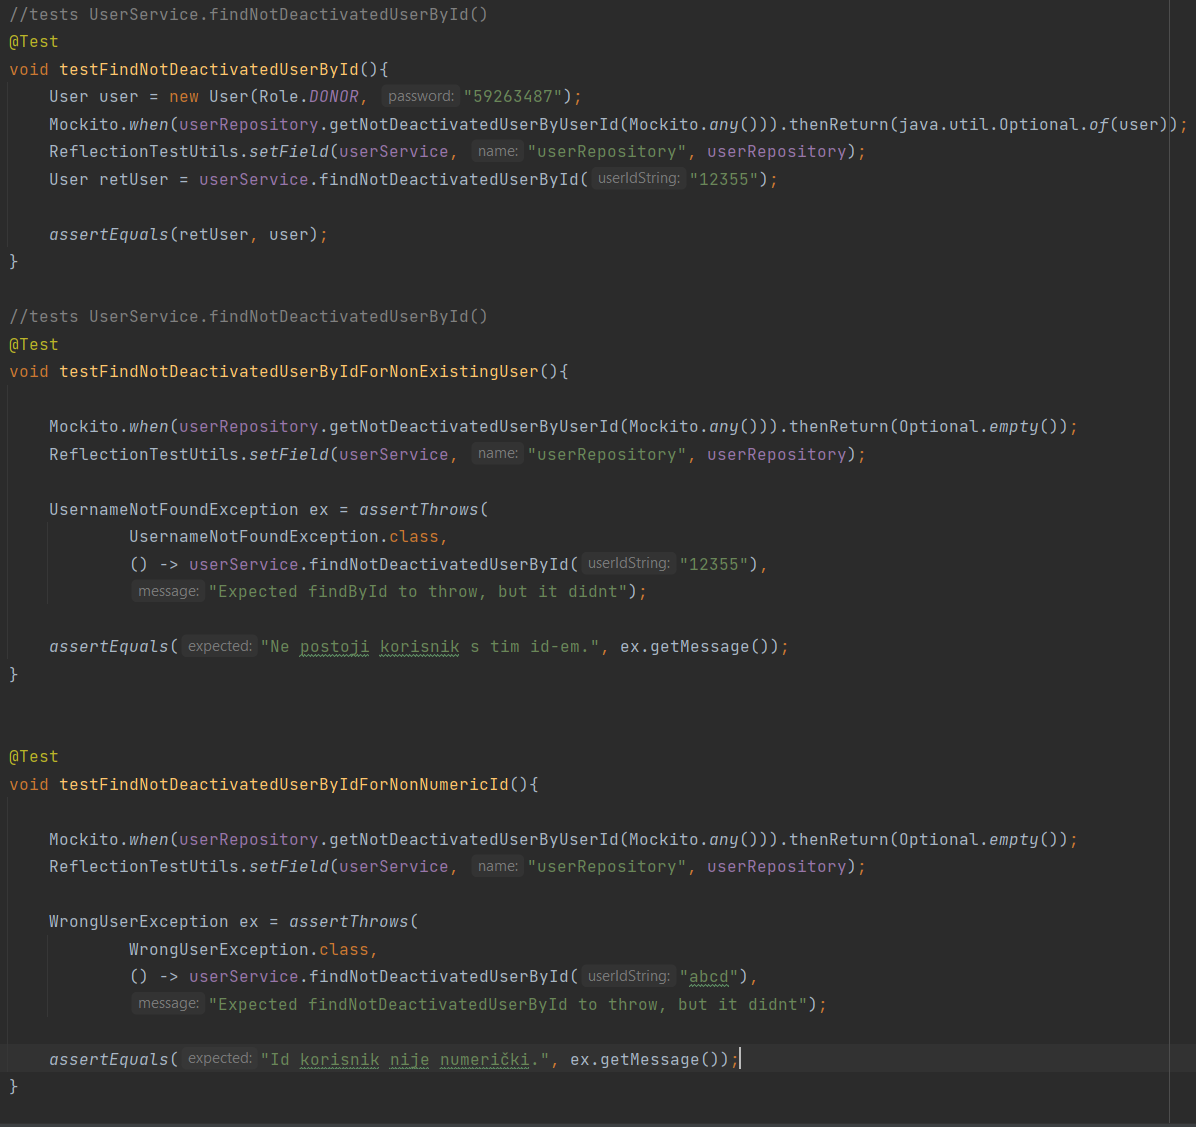
\includegraphics[scale=0.6]{slike/Tests/test1.png}
        			\centering
        			\caption{Testovi, prvi dio}
        			\label{fig:controller}
        		\end{figure}
        		\begin{figure}[H]
                    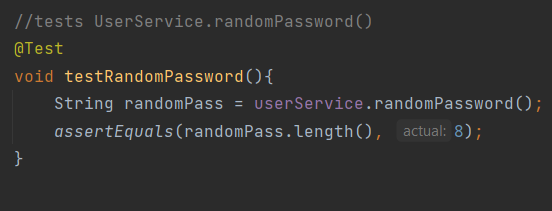
\includegraphics[scale=0.8]{slike/Tests/test2.png}
        			\centering
        			\caption{Testovi, drugi dio}
        			\label{fig:controller}
        		\end{figure}
        		\begin{figure}[H]
                    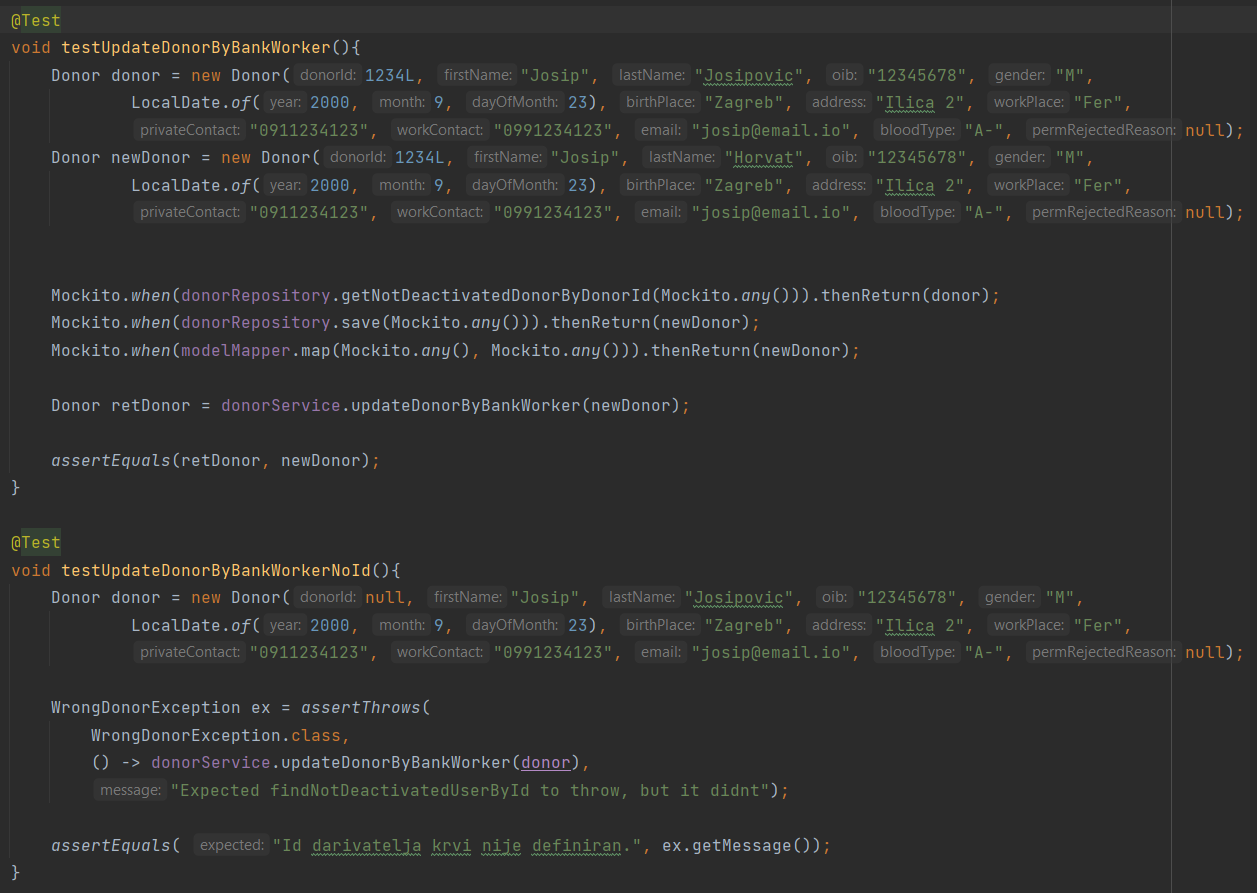
\includegraphics[scale=0.6]{slike/Tests/test3.png}
        			\centering
        			\caption{Testovi, treći dio}
        			\label{fig:controller}
        		\end{figure}
        		\begin{figure}[H]
                    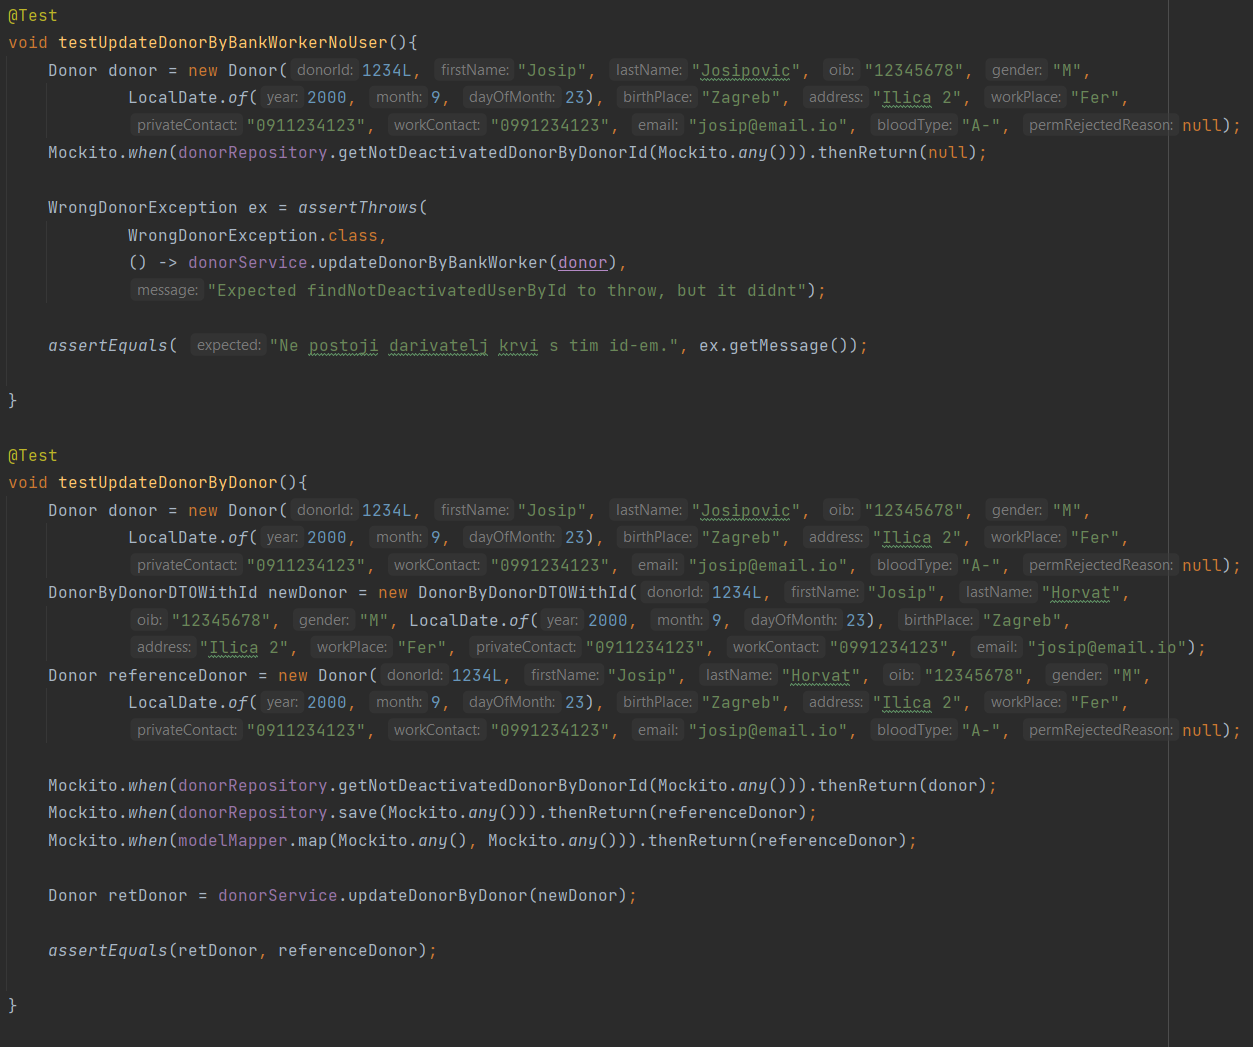
\includegraphics[scale=0.6]{slike/Tests/test4.png}
        			\centering
        			\caption{Testovi, četvrti dio}
        			\label{fig:controller}
        		\end{figure}
        		\begin{figure}[H]
                    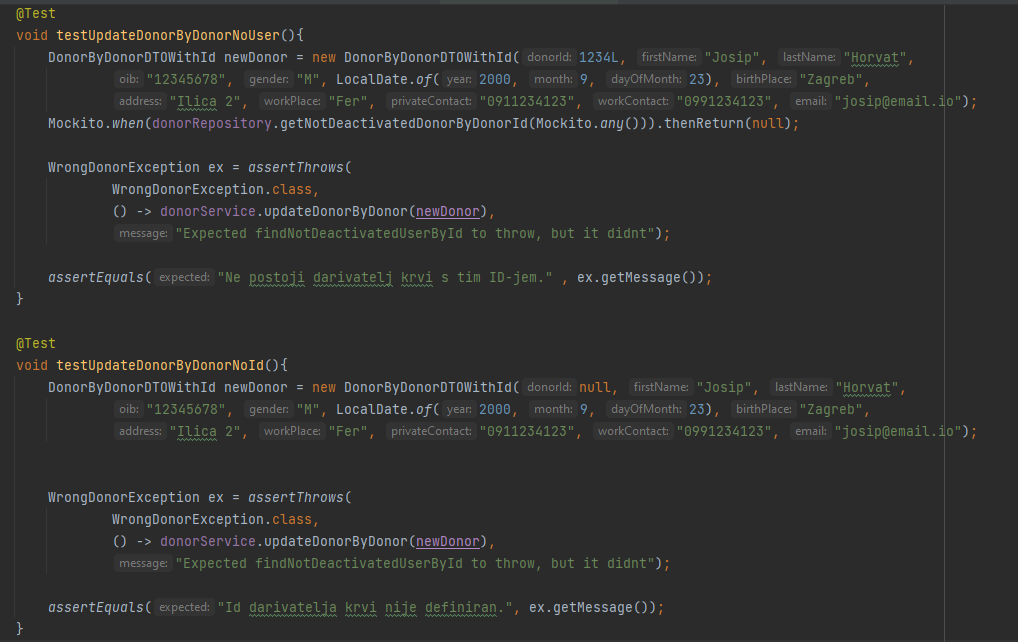
\includegraphics[scale=0.6]{slike/Tests/test5.png}
        			\centering
        			\caption{Testovi, peti dio}
        			\label{fig:controller}
        		\end{figure}
        		
        	%Na veliko zadovoljstvo svih sudionika, s
        	Svi testovi vraćaju prolaz te sve testirane funkcionalnosti rade. Slijedi dokaz:
			
			\begin{figure}[H]
                    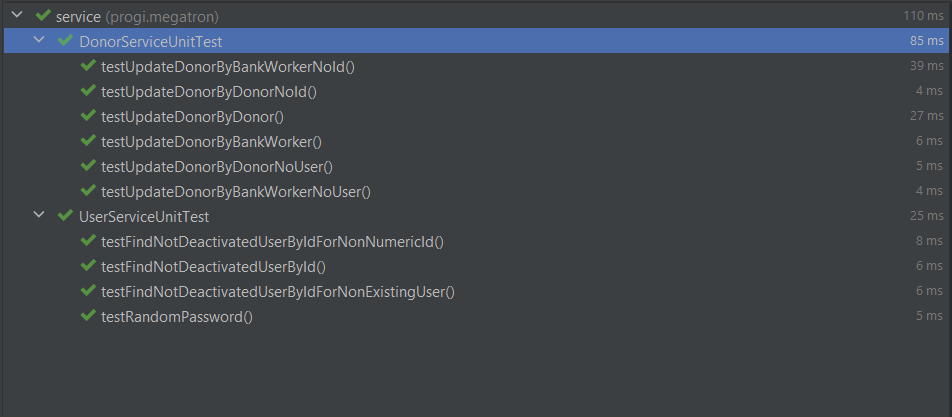
\includegraphics[scale=0.7]{slike/testovi rezultat.png}
        			\centering
        			\caption{Rezultati testiranja}
        			\label{fig:controller}
        		\end{figure}
			
			
			\eject
			\subsection{Ispitivanje sustava}
			
			 %\textit{Potrebno je provesti i opisati ispitivanje sustava koristeći radni okvir Selenium\footnote{\url{https://www.seleniumhq.org/}}. Razraditi \textbf{minimalno 4 ispitna slučaja} u kojima će se ispitati redovni slučajevi, rubni uvjeti te poziv funkcionalnosti koja nije implementirana/izaziva pogrešku kako bi se vidjelo na koji način sustav reagira kada nešto nije u potpunosti ostvareno. Ispitni slučaj se treba sastojati od ulaza (npr. korisničko ime i lozinka), očekivanog izlaza ili rezultata, koraka ispitivanja i dobivenog izlaza ili rezultata.\\ }
			 
			 
			 %\textit{Izradu ispitnih slučajeva pomoću radnog okvira Selenium moguće je provesti pomoću jednog od sljedeća dva alata:}
			 %\begin{itemize}
			 	%\item \textit{dodatak za preglednik \textbf{Selenium IDE} - snimanje korisnikovih akcija radi automatskog ponavljanja ispita	}
			 	%\item \textit{\textbf{Selenium WebDriver} - podrška za pisanje ispita u jezicima Java, C\#, PHP koristeći posebno programsko sučelje.}
			 %\end{itemize}
		 	%\textit{Detalji o korištenju alata Selenium bit će prikazani na posebnom predavanju tijekom semestra.}
			
			Koristeći Selenium IDE plugin za Chrome, provedeno je testiranje sustava. Korištena su četiri testa (slijede njihovi nazivi, opisi te rezultati):
			\begin{itemize}
			    \item 1. \textit{Prijava donora - odjava}:
			    Radi se o jednostavnom testu osnovne funkcionalnosti svakog korisnika. 
			    \begin{figure}[H]
                    
\includegraphics[scale=0.5]{slike/Tests/sistem1.png}
        			\centering
        			\caption{Rezultati prvog testa - profilna stranica prijavljenog korisnika}
        			\label{fig:controller}
        		\end{figure}
			    \item 2. \textit{Registracija (greška: Postojeći OIB)}:
			    Testira javljanje greške pri pravljenju računa sa već zauzetim OIB-om.
			    \begin{figure}[H]
                    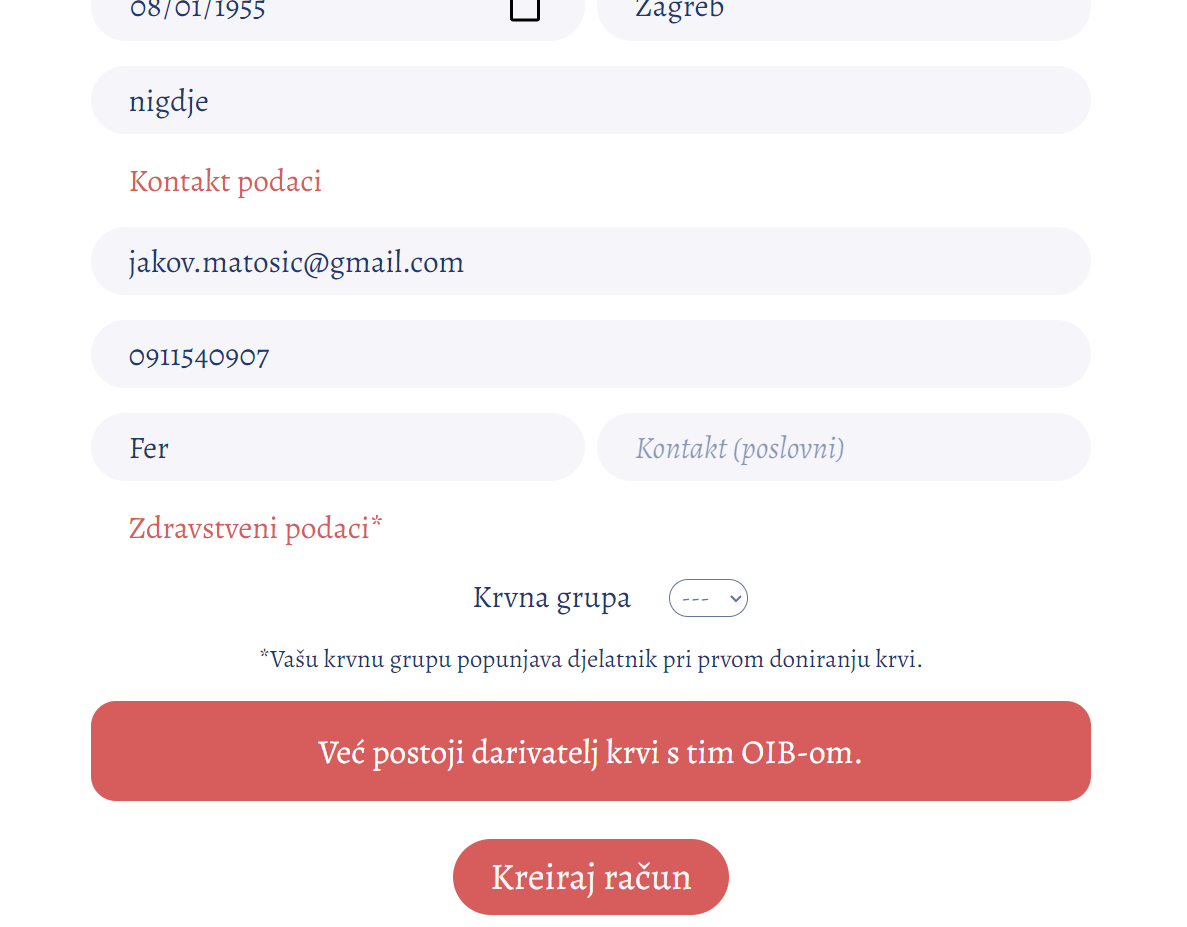
\includegraphics[scale=0.5]{slike/Tests/sistem2.png}
        			\centering
        			\caption{Rezultati drugog testa - greška zbog postojećeg korisnika}
        			\label{fig:controller}
        		\end{figure}
			    \item 3. \textit{prijava radnika - nova donacija (uključuje traženje donora) - odjava}:
			    Testira osnovnu funkcionalnost svakog radnika.
			    \begin{figure}[H]
                    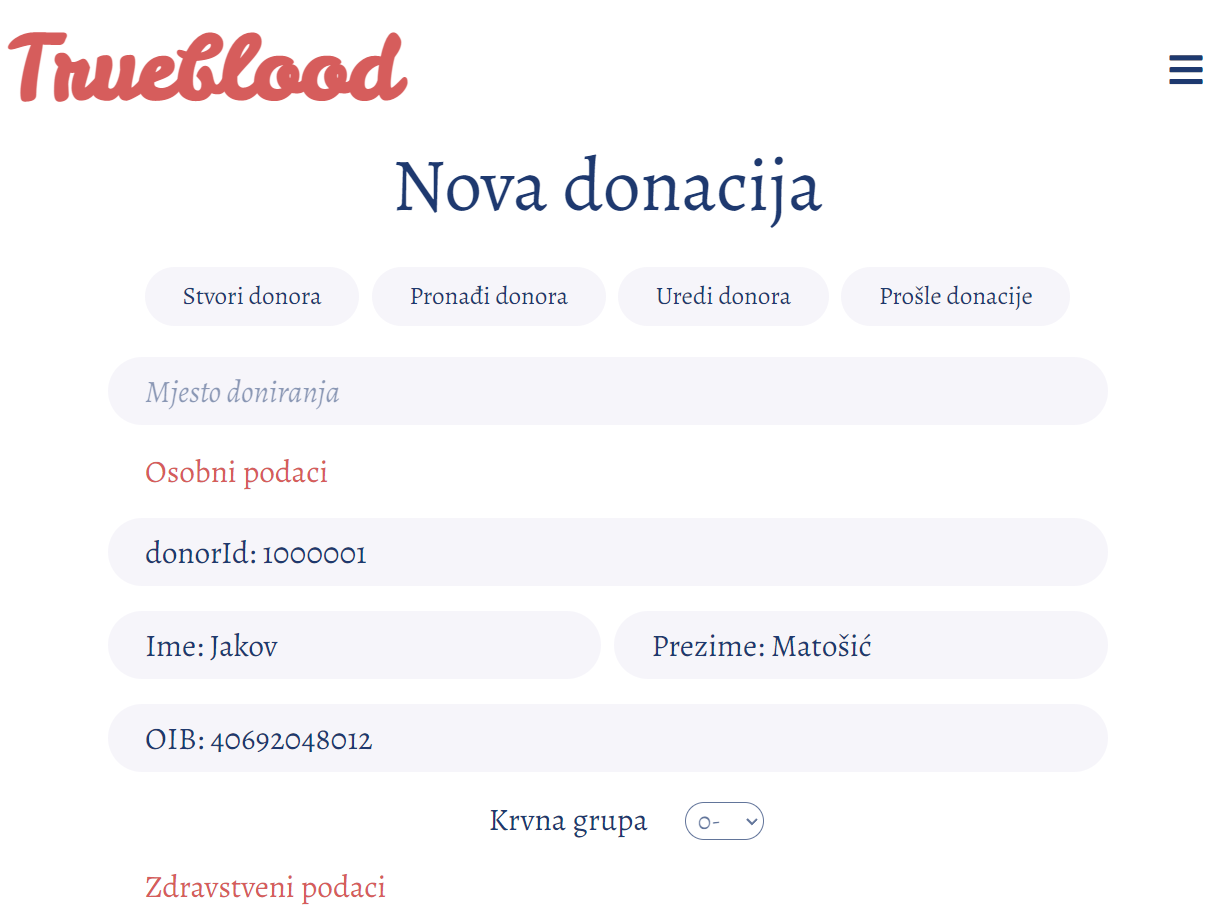
\includegraphics[scale=0.45]{slike/Tests/sistem3.png}
        			\centering
        			\caption{Rezultati trećeg testa - uspješno pronađeni korisnik i započeta donacija}
        			\label{fig:controller}
        		\end{figure}
			    \item 4. \textit{Prijava radnika - registracija novog donora sa greškama (krvna grupa nedefinirana, neispravna adresa e-pošte) - odjava}:
			    \begin{figure}[H]
                    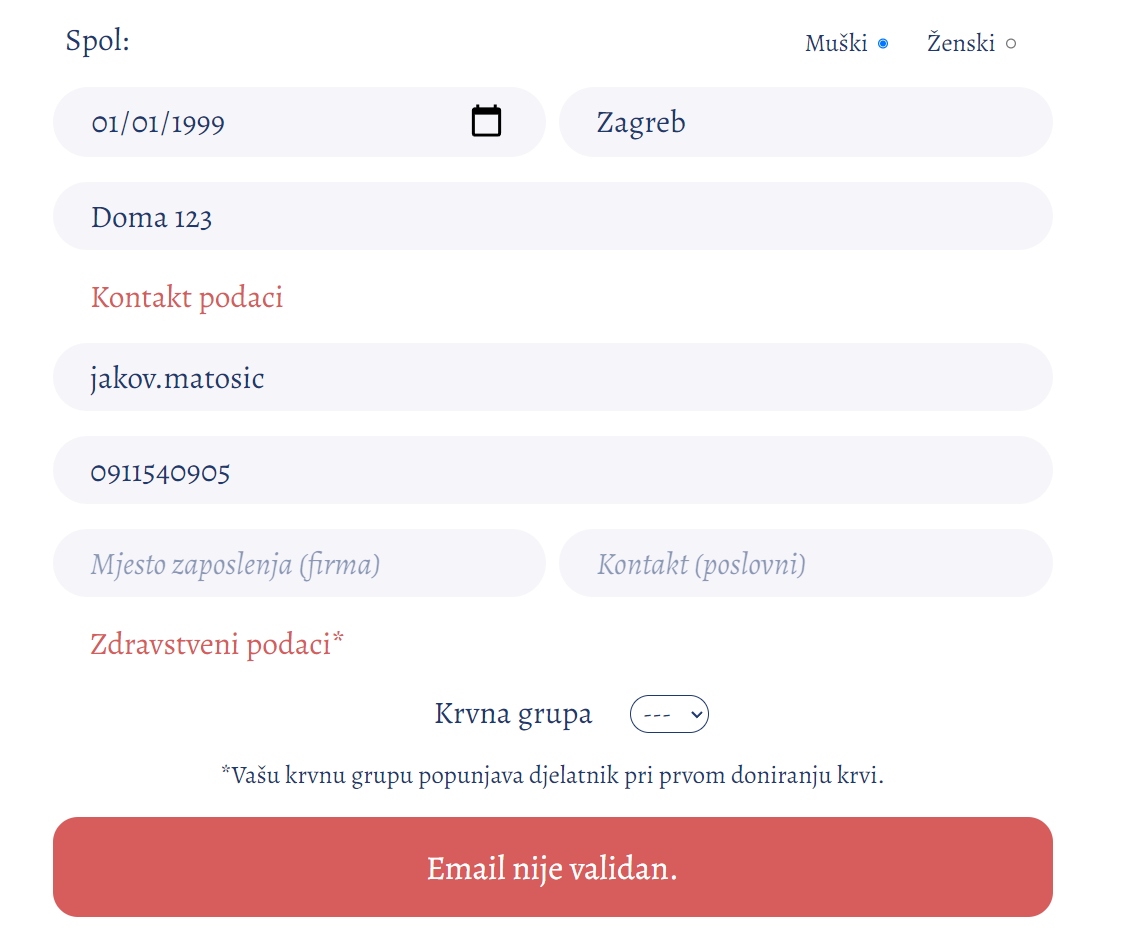
\includegraphics[scale=0.4]{slike/Tests/sistem4.png}
        			\centering
        			\caption{Rezultati četvrtog testa - greška}
        			\label{fig:controller}
        		\end{figure}
        		\begin{figure}[H]
                    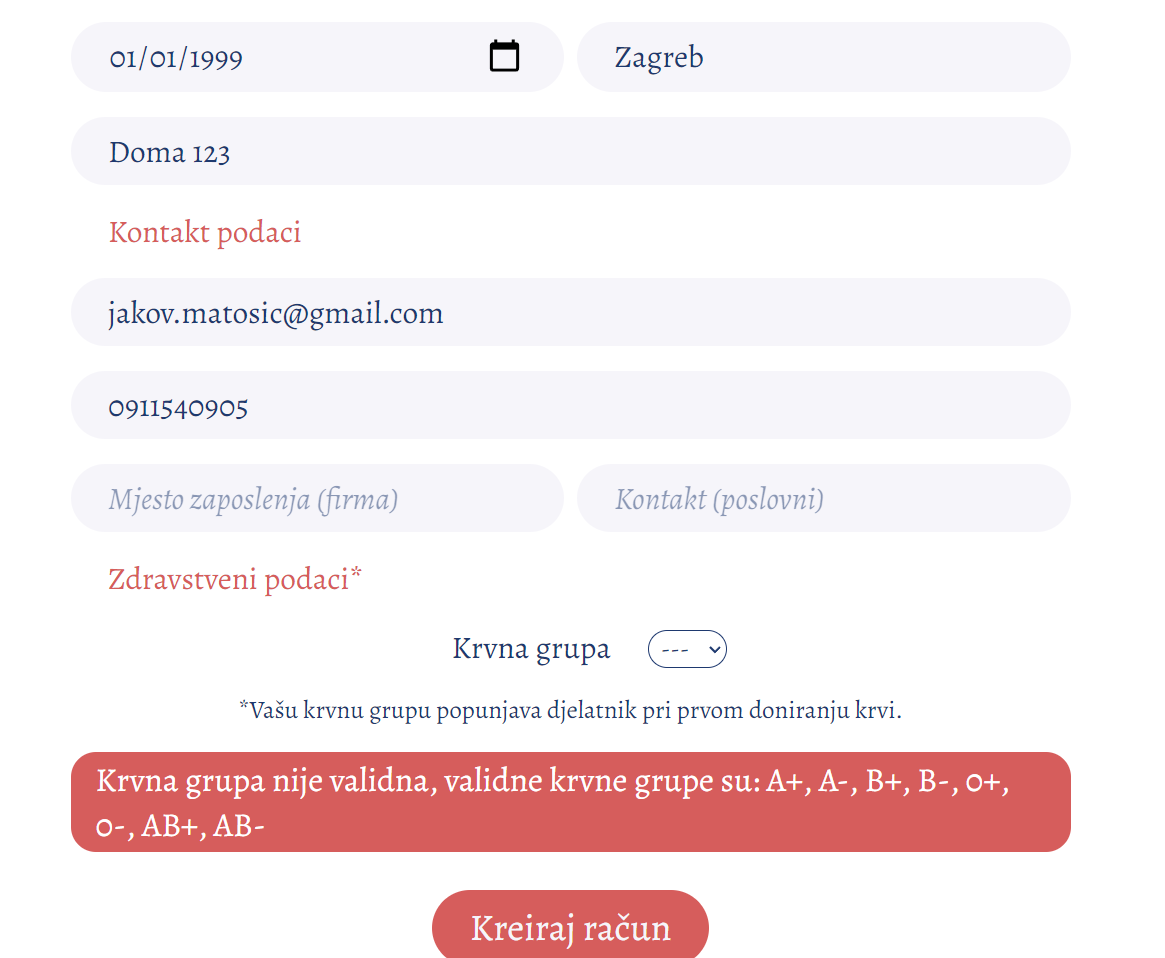
\includegraphics[scale=0.4]{slike/Tests/sistem5.png}
        			\centering
        			\caption{Rezultati četvrtog testa - greška}
        			\label{fig:controller}
        		\end{figure}
			\end{itemize}
			
			
			\eject 
		
		
		\section{Dijagram razmještaja}
			
% 			\textbf{\textit{dio 2. revizije}}
			
			 %\textit{Potrebno je umetnuti \textbf{specifikacijski} dijagram razmještaja i opisati ga. Moguće je umjesto specifikacijskog dijagrama razmještaja umetnuti dijagram razmještaja instanci, pod uvjetom da taj dijagram bolje opisuje neki važniji dio sustava.}
			 
			 \begin{figure}[H]             
    	        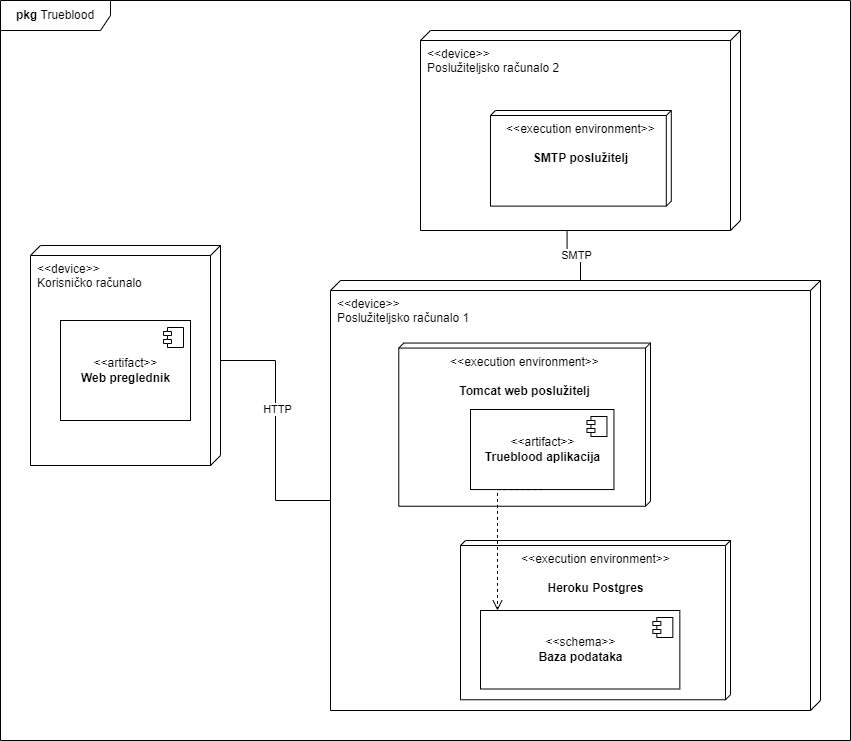
\includegraphics[scale=0.50]{slike/DR1_1.png}
            	\centering
            	\caption{Dijagram razmještaja}
            	\label{fig:dr}
            \end{figure}
            
            \par
            Dijagram razmještaja je UML dijagram koji opisuje topologiju sustava i prikazuje odnos sklopovskih i programskih dijelova. Korisničkom sučelju aplikacije pristupa korisnik sa svog računala putem web preglednika. HTTP vezom dohvaća i šalje podatke na poslužiteljsko računalo na kojem se nalaze web poslužitelj i poslužitelj baze podataka. Web poslužitelj također kontaktira SMTP poslužitelj kako bi se odvila funkcionalnost slanja mailova.
            
			
			\eject 
		
		\section{Upute za puštanje u pogon}
		
% 			\textbf{\textit{dio 2. revizije}}\\
		
			 %\textit{U ovom poglavlju potrebno je dati upute za puštanje u pogon (engl. deployment) ostvarene aplikacije. Na primjer, za web aplikacije, opisati postupak kojim se od izvornog kôda dolazi do potpuno postavljene baze podataka i poslužitelja koji odgovara na upite korisnika. Za mobilnu aplikaciju, postupak kojim se aplikacija izgradi, te postavi na neku od trgovina. Za stolnu (engl. desktop) aplikaciju, postupak kojim se aplikacija instalira na računalo. Ukoliko mobilne i stolne aplikacije komuniciraju s poslužiteljem i/ili bazom podataka, opisati i postupak njihovog postavljanja. Pri izradi uputa preporučuje se \textbf{naglasiti korake instalacije uporabom natuknica} te koristiti što je više moguće \textbf{slike ekrana} (engl. screenshots) kako bi upute bile jasne i jednostavne za slijediti.}
			
			
			 %\textit{Dovršenu aplikaciju potrebno je pokrenuti na javno dostupnom poslužitelju. Studentima se preporuča korištenje neke od sljedećih besplatnih usluga: \href{https://aws.amazon.com/}{Amazon AWS}, \href{https://azure.microsoft.com/en-us/}{Microsoft Azure} ili \href{https://www.heroku.com/}{Heroku}. Mobilne aplikacije trebaju biti objavljene na F-Droid, Google Play ili Amazon App trgovini.}
			
			\textbf{Instalacija i pokretanje Docker servisa}
			\begin{itemize}
    		    \item \text{Preuzmite prikladnu verziju \href{https://hub.docker.com/editions/community/docker-ce-desktop-windows/}{\textcolor{blue}{Dockera}} za svoj operacijski sustav}
			    \item Pokrenite Docker servis
			    
            	    \begin{minipage}{\linewidth}             
    	    	        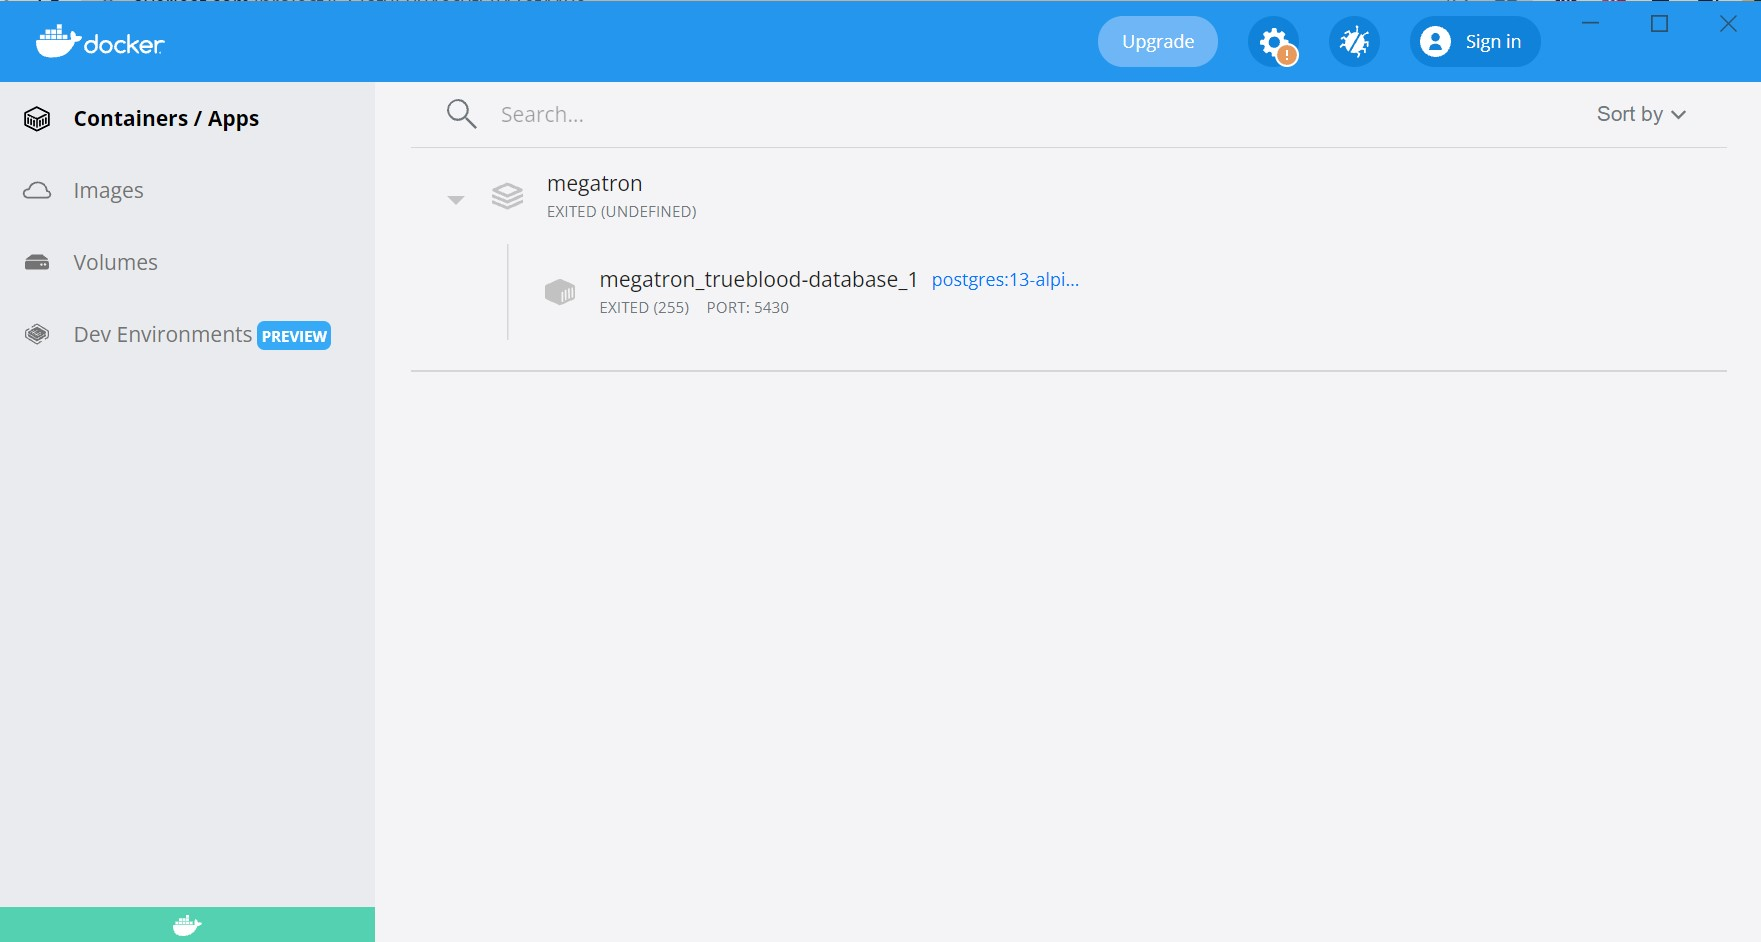
\includegraphics[scale=0.45]{slike/deploy/Docker1.jpg}
                    	\centering
                    	\captionof{figure}{Korisničko sučelje Dockera}
                    	\label{fig:DockerUI}
                    \end{minipage}
    	    	
    	    	\item U terminalu pozicioniranom u korijenskom direktoriju projekta upišite naredbu 

        	    	\begin{verbatim}
        $ docker-compose up
        	    	\end{verbatim}
        	    	
            	    \begin{minipage}{\linewidth}
                        \centering
                    	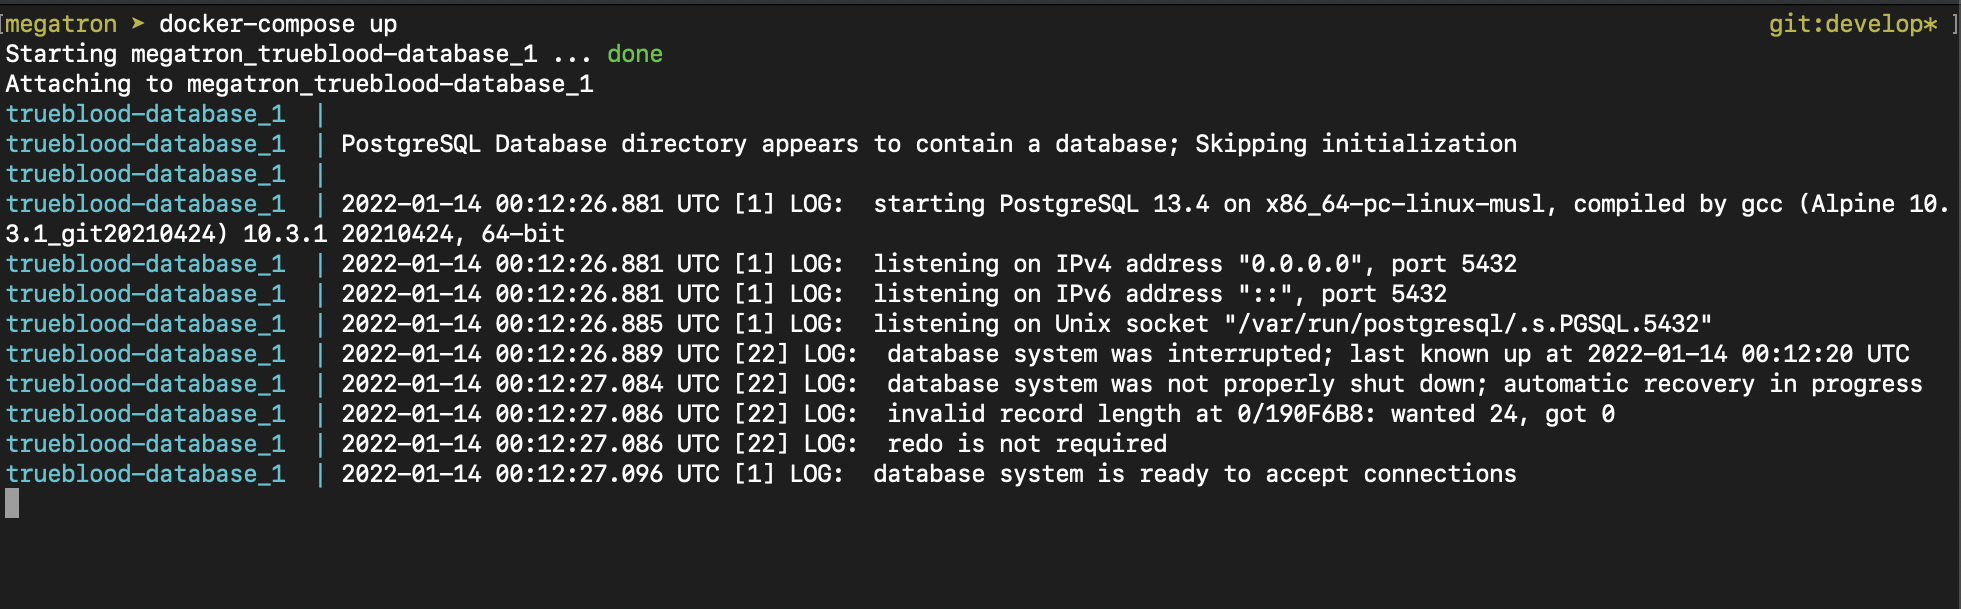
\includegraphics[scale=0.4]{slike/deploy/Docker2.png} %veličina slike u
                        \captionof{figure}{Pokretanje Docker spremnika}
                    \end{minipage}
        	    	%\begin{figure}
                    %	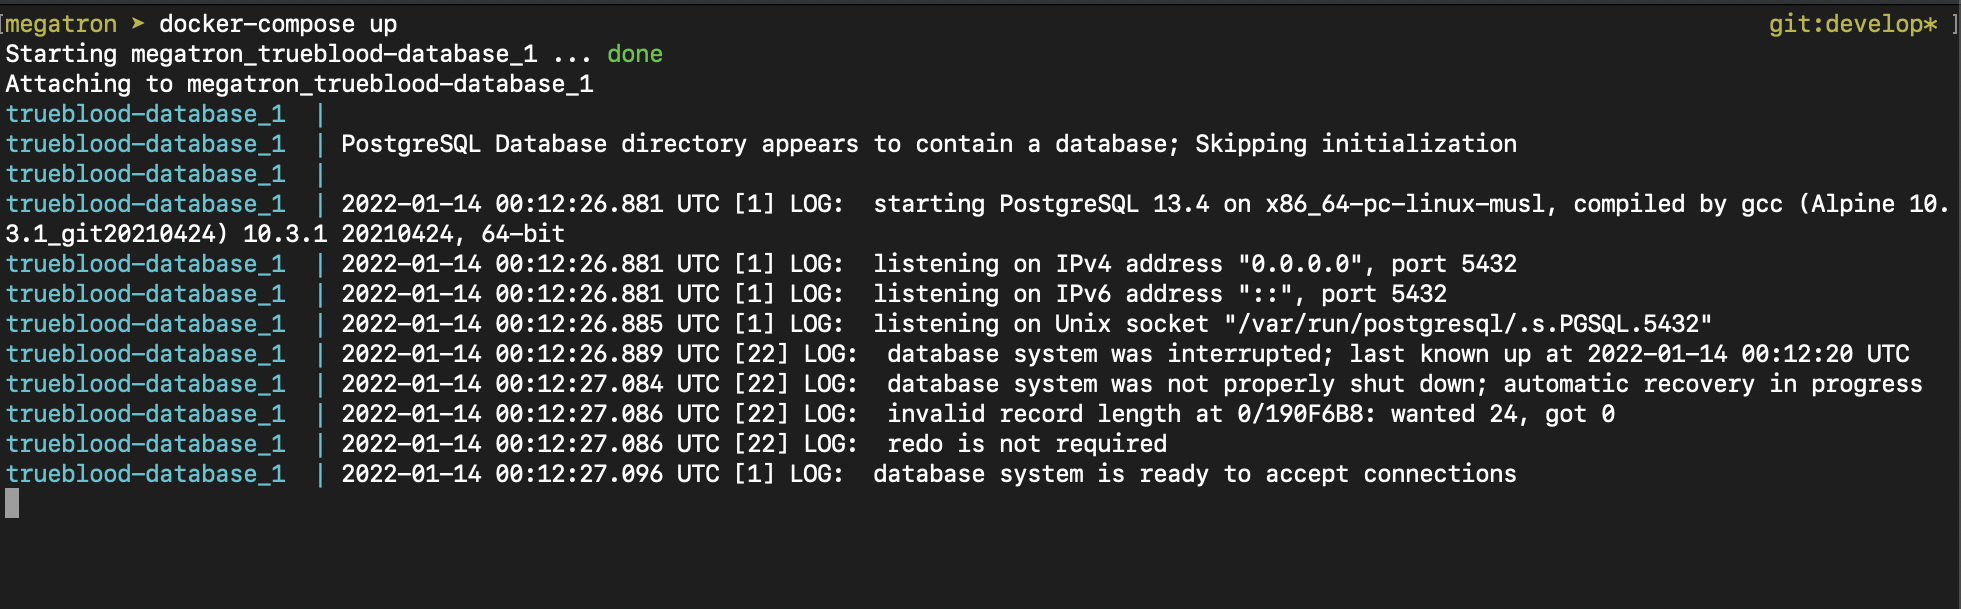
\includegraphics[scale=0.4]{slike/deploy/Docker2.png} %veličina slike u odnosu na originalnu datoteku i pozicija slike
            		%	\centering
            		%	\caption{Pokretanje Docker spremnika}
        		
        	    	%end{figure}
        	    
        	    \item Otvorite drugi terminal te u korijenskom direktoriju projekta upišite naredbu
        	    
            	    \begin{verbatim}
        $ psql -h localhost -p 5430 -d Trueblood -U admin
            	    \end{verbatim}
			    i password "admin"
			        
            	    \begin{minipage}{\linewidth}
                    	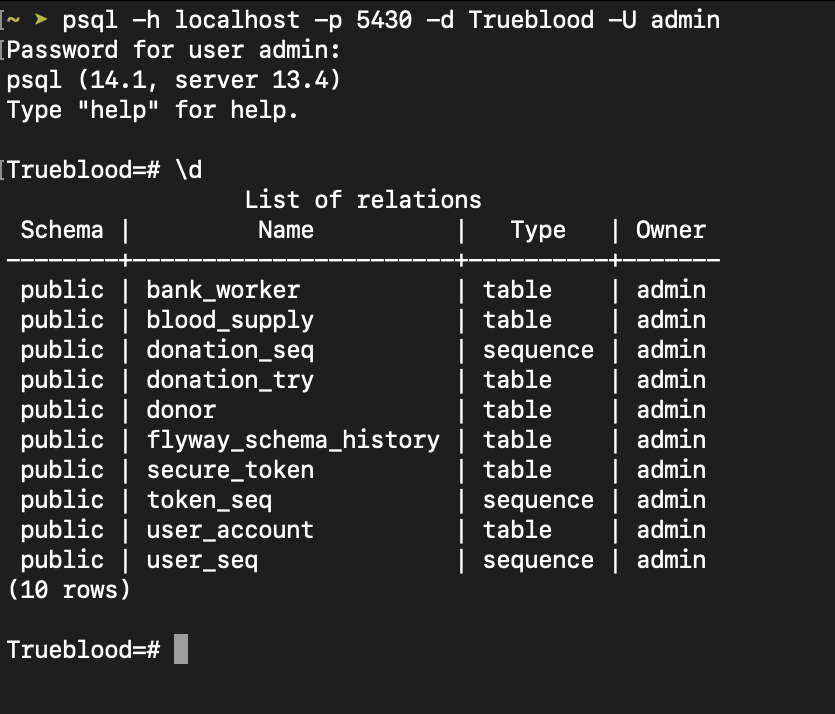
\includegraphics[scale=0.8]{slike/deploy/psql-primjer.png} %veličina slike u odnosu na originalnu datoteku i pozicija slike
            			\centering
            			\captionof{figure}{Spajanje na bazu pomoću alata PSQL}
        		        \label{fig:psql}
                    \end{minipage}
			    
			\end{itemize}
			\eject
			
			\textbf{Postavljanje frontenda}
			    \begin{itemize}
			        \item Preuzmite i instalirajte Node.js i			         \href{https://docs.npmjs.com/downloading-and-installing-node-js-and-npm}{\textcolor{blue}{npm}}
			        
			        \item Preuzmite yarn narebom 
			        \begin{verbatim}
			            $ npm install --global yarn
			        \end{verbatim}
			        
			        \item Pokretanjem naredbe
			        \begin{verbatim}
			            $ yarn install
			        \end{verbatim}
			        instalirat će se potrebni paketi
			        
			        \item Razvojni poslužitelj (engl. \textit{development server}) pokreće se naredbom 
			        \begin{verbatim}
			            $ yarn start
			        \end{verbatim}
			        
            	    \begin{minipage}{\linewidth}
                    	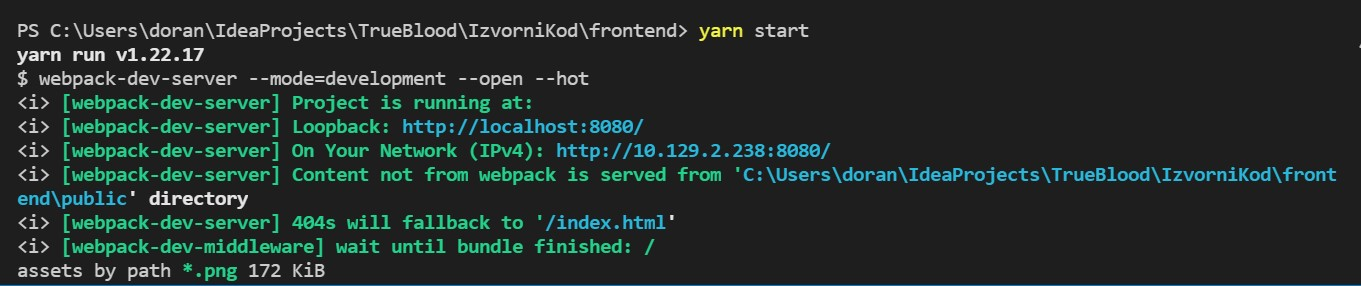
\includegraphics[scale=0.6]{slike/deploy/yarn-start.jpg} %veličina slike u odnosu na originalnu datoteku i pozicija slike
            			\centering
            			\captionof{figure}{Pokretanje razvojnog poslužitelja}
        		        \label{fig:yarnstart}
                    \end{minipage}
			        
			    \end{itemize}
			\eject
			    
			\textbf{Javno puštanje aplikacije u pogon}
    			\begin{itemize}
    			    \item Napravite \href{https://signup.heroku.com/}{\textcolor{blue}{Heroku korisnički račun}}
    			    \item Instalirajte \href{https://devcenter.heroku.com/articles/heroku-cli}{\textcolor{blue}{Heroku CLI}}
    			    \item Koristeći naredbu 
    			    \begin{verbatim}
    			        $ heroku login
    			    \end{verbatim}
    			    pokrenite postupak autorizacije
			    \end{itemize}
    			 %\eject
    			 \textbf{Primjeri korištenja Heroku alata} \newline
    			 \textit{Navedeni primjeri mogu se koristiti i s trueblood-fe}
    			 \begin{itemize}
    			 \item Za ponovno pokretanje aplikacije upišite naredbu
    			 \begin{verbatim}
    			     $ heroku restart --app trueblood-be
    			 \end{verbatim}
    			 \item Za uvid u zapisnik aplikacije
    			 \begin{verbatim}
    			    $ heroku logs --tail --app trueblood-be
    			 \end{verbatim}

                \item Pregled trenutnih build radnji
                \begin{verbatim}
        $ heroku builds --app trueblood-be
                \end{verbatim}
                
                \item Povezivanje s bazom pokreće se naredbom
                \begin{verbatim}
        $ heroku pg:psql --app trueblood-be
                \end{verbatim}
                \textit{ova naredba nije dostupna za trueblood-fe}
    			\end{itemize}
    		Status cjevovoda moguće je provjeriti na GitLabu. U slučaju podbacivanja cjevovoda te dobivanja poruke \textit{Your account has reached its concurrent builds limit} u zapisniku aplikacije, potrebno je ponovno pokrenuti aplikaciju.
			\eject 